\begin{figure}[H]
    \centering
    \begin{subfigure}{0.48\columnwidth}
        \centering
        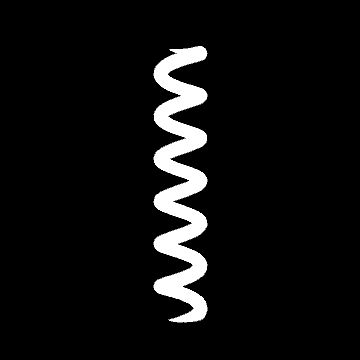
\includegraphics[width=\columnwidth]{figures/slit shape.png} % first figure itself
        \caption{slit shape of a helix generated by projecting a 3d helix on to a plane}
        \label{fig:expansion slit shape}
    \end{subfigure}\hfill
    \begin{subfigure}{0.48\columnwidth}
        \centering
        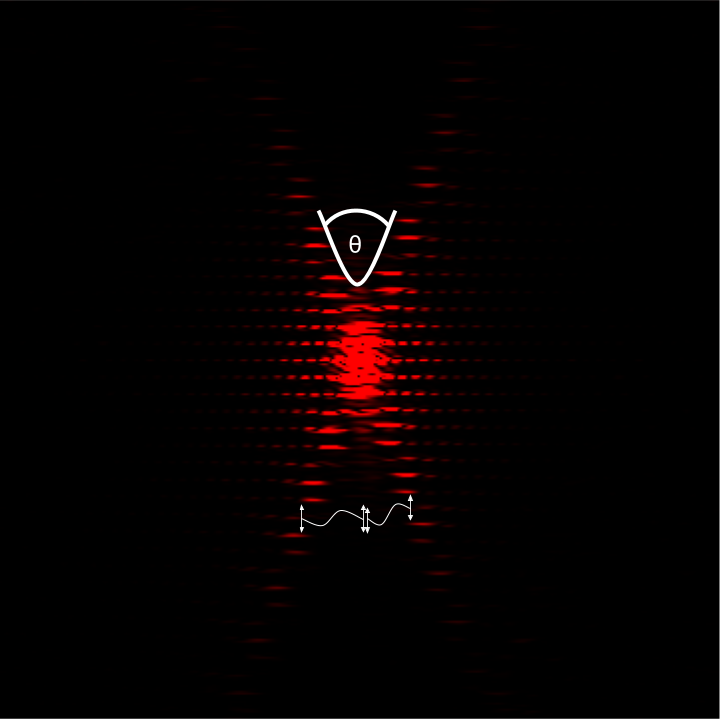
\includegraphics[width=\columnwidth]{figures/interference pattern.png} % second figure itself
        \caption{magnitude square of discrete fourie transform of slit shape shown in \ref{fig:expansion slit shape}}
        \label{fig:expansion interference simulation}
    \end{subfigure}
    \begin{subfigure}{0.48\columnwidth}
        \centering
        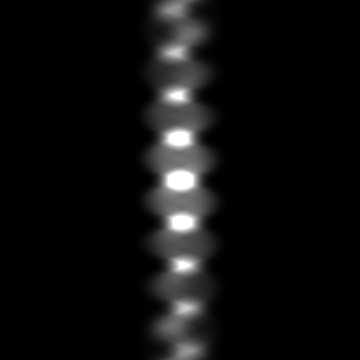
\includegraphics[width=\columnwidth]{figures/reverse fourie transform.png}
        \caption{inverse fourie transform of \ref{fig:expansion interference simulation} showing
        the inverse fourie transform of the square of the fourie transform of \ref{fig:expansion slit shape}}
        \label{fig:expansion inverse fourie transform}
    \end{subfigure}
    \begin{subfigure}{0.48\columnwidth}
        \centering
        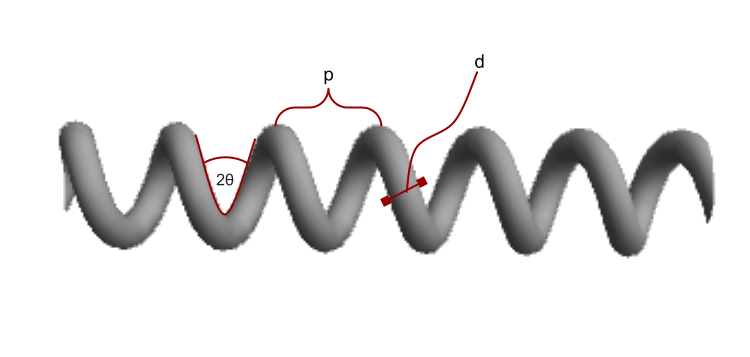
\includegraphics[width=\columnwidth]{figures/spring parameters illustration.png}
        \caption{spring parameters illustration}
        \label{fig:spring parameters illustration}
    \end{subfigure}

    \label{fig:expansion theory illustrations}
\end{figure}
